% 1987 年全国卷文科第八题：y=sin 2x 的示意图
\begin{tikzpicture}[scale=0.72,>=stealth,font=\small]
  \draw[->] (-1.9,0)--(3.55,0) node[below right] {$x$};
  \draw[->] (0,-1.45)--(0,1.55) node[left] {$y$};
  \draw[thick,domain=-1.75:3.25,samples=160,smooth]
    plot (\x,{sin(deg(2*\x))});
  \node[below] at (-1.57,0) {$-\dfrac\pi2$};
  \node[below right] at (0.05,0) {$O$};
  \node[below] at (1.57,0) {$\dfrac\pi2$};
  \node[below] at (3.14,0) {$\pi$};
  \node[left] at (0,1) {$1$};
  \node[left] at (0,-1) {$-1$};
\end{tikzpicture}
